%!TEX root = ../thesis.tex
%*******************************************************************************
%****************************** Second Chapter *********************************
%*******************************************************************************

\chapter{Quantifying received dose errors introduced by modelling approximations in reinforced concrete shielding}
\label{chap:homogenisation}

\ifpdf
    \graphicspath{{Chapter2/Figs/Raster/}{Chapter2/Figs/PDF/}{Chapter2/Figs/}}
\else
    \graphicspath{{Chapter2/Figs/Vector/}{Chapter2/Figs/}}
\fi

% ITER report is robust and actually quite well written, use as base
% Check with Roddy I can use material from this report
% Need some introductory material on spatial homogenisation:
%     Raoul's report?
%     Wider literature
% Additional figures which might be nice:
%     Nice SDDR photon ratio
%     Interpolated (time, E, ratio) heatmap

\section{Outline}
This chapter looks at %%%

%INTRODUCTION
\section{Introduction}
The ITER nuclear fusion experiment will begin DT operation in the 2030s. At 500MW fusion power the source rate of 14.1MeV neutrons will approximately $1.8\times10^{20}$ s\textsuperscript{-1}. For comparison, JET's maximum source rate to date is 30 times less. But the real difference is in the fluence. JET's lifetime neutron budget is $2\times10^{21}$ \cite{Lobel08}, or 10 seconds of operation for ITER-DT. The ITER life-time budget is approximately $3\times10^{27}$ neutrons.

Designing a complex device such as a superconducting tokamak to operate in this radiation environment is a particularly challenging aspect of the ITER project. Care must be taken both to shield sensitive components like semiconductor devices from Single Event Effects (SEE) and to prevent excessive nuclear heating in large systems like the superconducting coils. The high flux and fluence of high energy neutrons means activation in areas like the Neutral Beam (NB) cells and in the Tokamak Cooling Water System (TCWS) will be significant. And of course, gamma from these activated components, and the prompt radiation of a thermonuclear plasma must be shielded against to protect the workforce operating and maintaining the plant.

Quantifying the absorbed dose to radiation sensitive components, or the equivalent dose to personnel requires crafting a computer model of the problem and typically making a series of assumptions and simplifications in the process. For reinforced concrete radiation shields, this often entails either homogenising the rebar with the concrete, or even neglecting the presence of rebar entirely. This process introduces systematic error into the reported solution of the problem. However, uncertainty in an answer is not solely from geometrical simplification, but also from other input data. Cross-section, secondary particle and decay data can be flawed or missing and materials compositions can be incorrect. In the case of reinforced concrete, the water and therefore hydrogen content is uncertain. This is because not only can the water content change from batch to batch, but also over time (during the plant lifetime) for a given batch.

\subsection{Radiation shielding}
% Lit review.

\subsection{Spatial homogenisation}
% Lit review.

\subsection{ITER bioshield}

%METHOD
\section{Method}
The modelling simplification under investigation is that of spatial homogenisation and how it affects doses to workers, whether prompt or delayed. It is theorised that any errors incurred by this modelling approximation will be functions of geometry and material composition. For each set of variables interrogated, at least two simulations will be performed. One will have a high-fidelity model of the real-world problem geometry with reinforcing bar and stirrup rods faithfully reproduced. The other will smear the rebar across the concrete, homogenising the two materials into one with a density equal to the mass weighted sum of the concrete and steel constituents. 

Simulations employing realistic ITER source particle distributions will tally transmitted or `leakage' fluence at the rear of the shielding walls in both cases. This permits comparison between the modelling approximation and the higher-fidelity simulation.

The implications of spatial homogenisation prove to be different for on-load and shut-down (activated) dose rates. It is helpful to consider them seperately. The following two sections detail the methods for determining these two dose rates.

\subsection{Prompt neutron \& gamma radiation}
Determining the dose to personnel beyond a wall requires knowledge of the radiation fluxes there. The on-load gamma flux $\phi_{\gamma}(x,y,z,E,t)$ and neutron flux, $\phi_{n}(x,y,z,E)$, can be computed with Monte Carlo techniques, spawning neutrons from a prerecorded source distribution, $P(x,y,z,E,\Omega)$ at a particular point with a given energy and angle. These particles may propagate through the wall, scattering, being absorbed, exciting nuclei (which later relax through radiative emission) and perhaps leaking out of the back of the shield wall. Tallying this leakage flux of neutrons and photons is the main task of calculating a dose due to radiation.

\subsubsection{Model geometry}
The heterogeneous, realistic wall is constructed of a large concrete block, with two meshes of rebar, one buried below each face. The distance from wall exterior to rebar is known as the cover depth. Connecting the two meshes are a small number of narrow gauge `stirrup' bars. The homogeneous model is the same external dimensions and total mass as the heterogeneous one, but without an internal steel structure and with homogenised materials.

A Python program has been written to take wall thickness, cover depth and other parameters as input variables to construct a corresponding MCNP model. This model utilises lattices to construct the repeated features of the reinforced concrete wall. The concrete block dimensions are $(x, y, z) = (10, y, 10)$ where $y$ is the wall thickness. Embedded within the block are the major two meshes of steel reinforcement. These meshes are always constructed with 200mm spaced rebar extendeding in both the x and z directions \cite{Perez2014}. The meshes are buried a small cover depth from the two $y$-perpendicular surfaces of the wall. Tying the two meshes together are some thinner `stirrup' bars extending in the y direction, with $\approx 4m^{-2}$ of wall face \cite{Perez2014}. A particular level of reinforcement may be referred to as 16HB200, i.e. 16mm diameter rebar, at 200mm spacing.

Simulations were run for the following wall thicknesses: 30, 50, 80, 120 \& 210 cm. For each case, the fraction of total wall mass as steel was kept constant at 4.45\%. This was achieved by increasing the rebar diameter, noting the relationship shown in equation~\ref{eq:rebar}. 

\begin{equation}
  \label{eq:rebar}
  \frac{d^{2}_{r}}{t_{w}} \propto f_{s}
\end{equation}

That is, the rebar diameter, $d_{r}$ squared divided by the wall thickness, $t_{w}$ is proportional to the steel fraction, $f_{s}$. The value of 4.45\% was chosen as this is a typical value computed from the description of reinforcement and dimensions in \cite{Perez2014}. 

Material compositions, wall widths, rebar arrangements and steel fractions have been determined from ITER drawings and specifications for concrete walls in the tokamak building. The work has been conducted with a moderated ITER DT fusion neutron source spectrum. The results should give a good idea of the implications of the homogeneous modelling approximation at ITER but also more generally given the standard civil engineering design of the reinforced concrete walls.

% column span figure
\begin{figure}[h]
  \figuretitle{Homogenising reinforced concrete}
  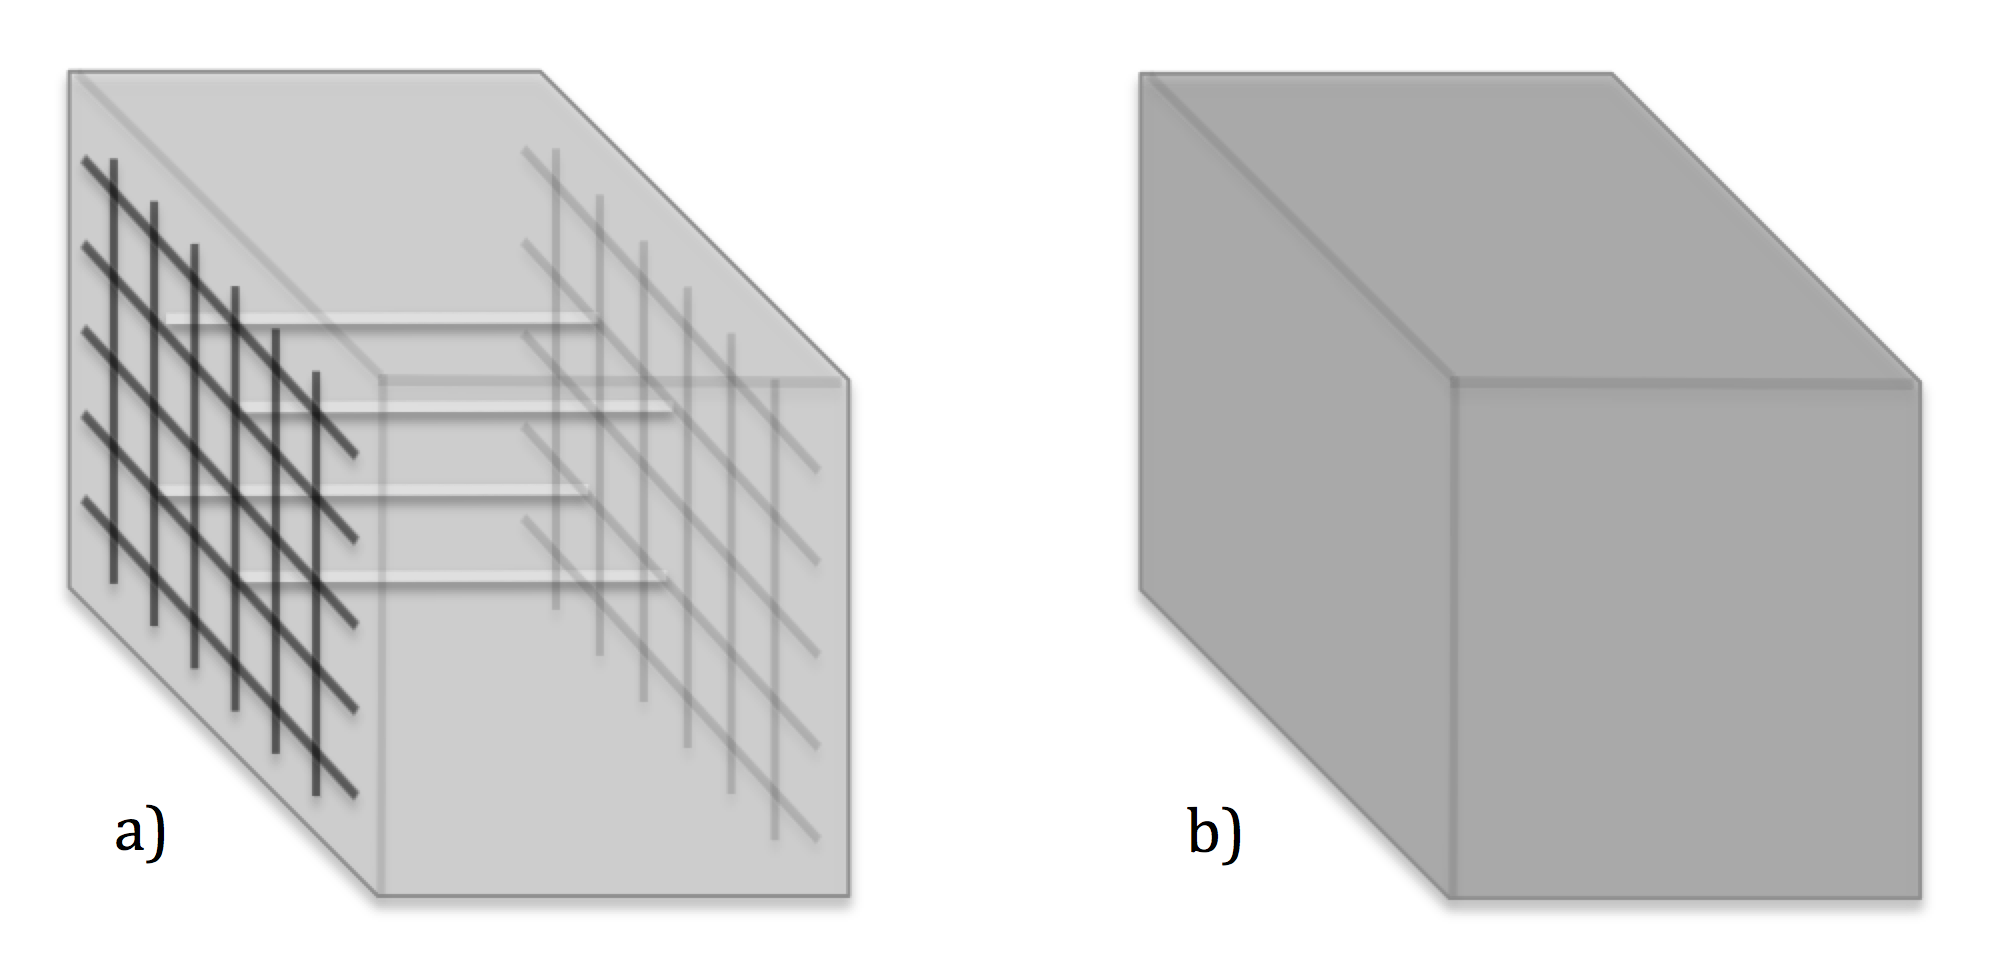
\includegraphics[width=\textwidth]{wall_diagram}
  \caption{The two modelling approaches considered in this investigation. a) Heterogeneous, where the steel reinforcing bar and stirrups are explicitly modelled. b) Homogeneous, where the mass of rebar is 'smeared' through the concrete. The new homogenised material has a greater density than plain concrete, conserving mass.}
  \label{fig:wall_diagram}
\end{figure}

\subsubsection{Materials}
Although much of the investigation will be by comparing values for homogeneous and heterogeneous responses, it is still important to supply the most accurate input information possible for the simulations. All the compositions that follow were mixed using the PyNE python package \cite{Pyne18} employing natural abundance for isotopic distributions.

\paragraph{Concrete}
The density of concrete used is 2.2g cm\textsuperscript{-3} \cite{Jakhar16}. The composition is shown in table~\ref{tab:concrete}. 

\begin{table}[H]
  \centering
  \begin{tabu} to 0.3\textwidth {X X}
    \toprule
    Element   &   \% weight \\
    \midrule
    H & 0.56 \\
    O & 49.75 \\
    Na & 1.71 \\
    Mg & 0.26 \\
    Al & 4.69 \\
    Si & 31.47 \\
    S & 0.13 \\
    K & 1.92 \\
    Ca & 8.28 \\
    Fe & 1.24 \\
    \bottomrule
  \end{tabu}
  \caption{Concrete composition \% weight from \cite{Jakhar16}. The H content may be overestimated in this mixture. Sampling suggests it may be as low as 0.2\%wt \cite{Aramburu16}. The consequences of such an deviation are substantial and were investigated in work not presented here.}
  \label{tab:concrete}
\end{table}

\paragraph{Steel}
The density of steel used for rebar is 7.85g cm\textsuperscript{-3} \cite{BSsteel05}. The steel minor constituents Cu, Mn, Cr, Mo, V and Ni are not specified in \cite{BSsteel05} however the CEV (Carbon Equivalent Value) is given, a figure for quantitatively comparing the `weldability' of steels. The CEV formula was used to determine likely \% fractions of the aforementioned elements, giving a material composition as shown in table~\ref{tab:steel}.

\begin{table}[H]
  \centering
  \begin{tabu} to 0.3\textwidth {X X}
    \toprule
    Element & \% weight \\
    \midrule
    Fe & 97.24 \\
    C & 0.22 \\
    P & 0.05 \\
    S & 0.05 \\
    N & 0.012 \\
    Mn & 0.56 \\
    Cr & 0.16 \\
    Mo & 0.16 \\
    V & 0.16 \\
    Ni & 0.7 \\
    Cu & 0.7 \\
    \bottomrule
  \end{tabu}
  \caption{Steel composition \% weight from \cite{BSsteel05}.}
  \label{tab:steel}
\end{table}

\subsubsection{Radiation sources}
The effect of spatial homogenisation is considered for both neutron and photon radiation, hence likely distributions are required for both particle types.

No particle direction information was available, so it was assumed that all particles are born travelling perpendicular to the radiation shield. It was reasoned that this is a conservative assumption, liable to increase the discrepancy between heterogeneous and homogeneous approaches as the heterogeneous model has features (the stirrup bars) which are aligned with this initial particle direction.

% column span figure
\begin{figure}[H]
  \figuretitle{ICRP74 flux to dose factors}
  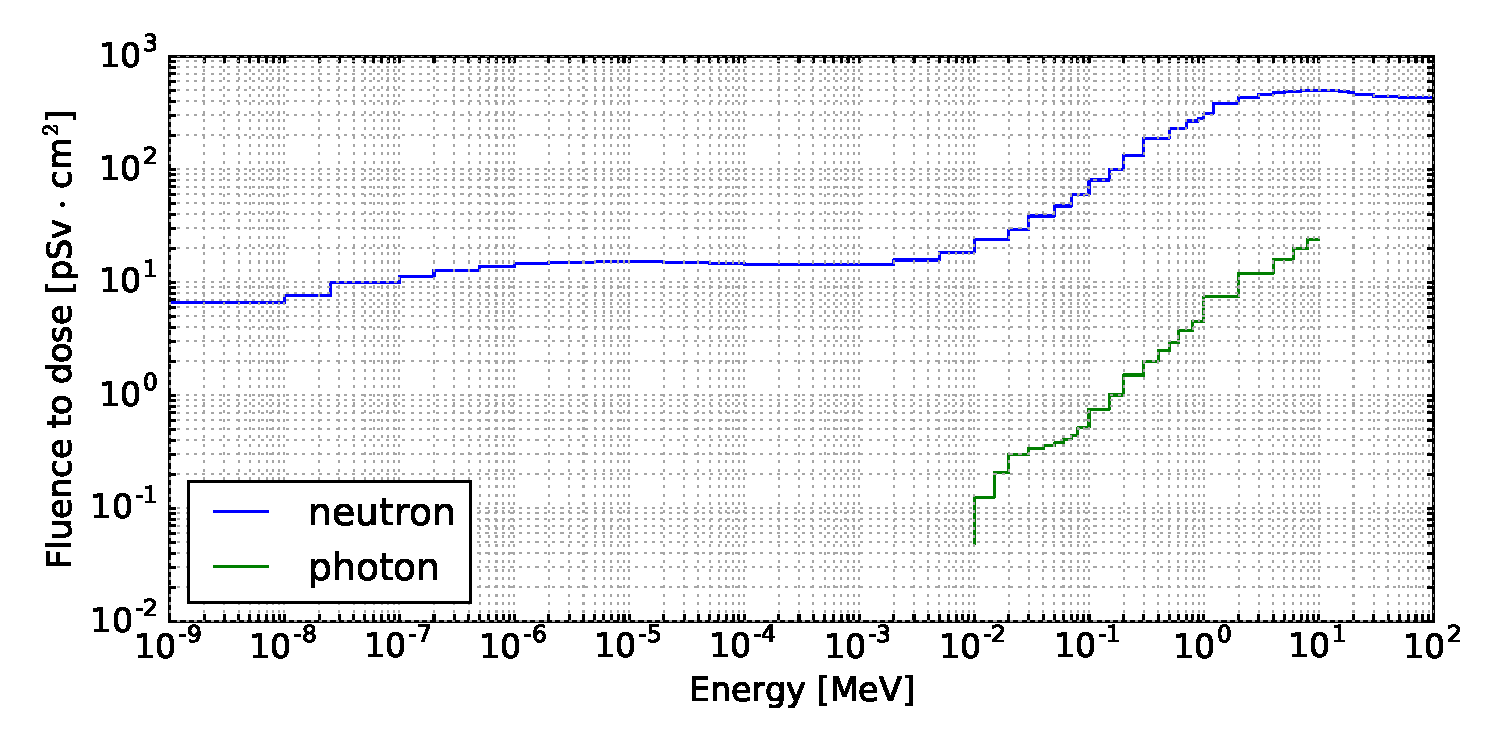
\includegraphics[width=\textwidth]{icrp74}
  \caption{The flux to dose conversion factors for neutron and photon exposure.}
  \label{fig:icrp74}
\end{figure}

The effective dose to humans is a function of the energy and type of radiation. It takes into account the varying susceptibilities of different tissues in the human body. For radiation protection, this is the typical figure quoted when specifying a dose rate. Where required, translation from fluence or flux to dosea or dose-rate respectively is by functions as shown in figure \ref{fig:icrp74}.

\paragraph{Neutron}
The neutron source spectrum was obtained in previous work by \citeauthor{Jakhar16} and is shown below as \ref{fig:src_spectra}. The location tallied for this particle spectrum was behind a ITER neutral beam assembly, of neutrons incident upon the shield wall behind. In the ITER plant this area will receive an elevated flux over other areas of the bioshield due to the penetrations from neutral beam injectors into the plasma chamber. The neutron spectrum was provided in the 175 VITAMIN-J group structure. Unfortunately this group structure provides very little information about the fine structure of the thermal neutron distribution below 0.1 eV. This is a deficiency in this study as the source spectrum is heavily thermalised. For the radiation transport simulations, no neutron source rates or wall loadings were specified. Instead, results were reported per source neutron. Many of the results later presented are ratios of the same quantity and hence unitless. 

% column span figure
\begin{figure}[H]
  \figuretitle{Neutron source spectrum}
  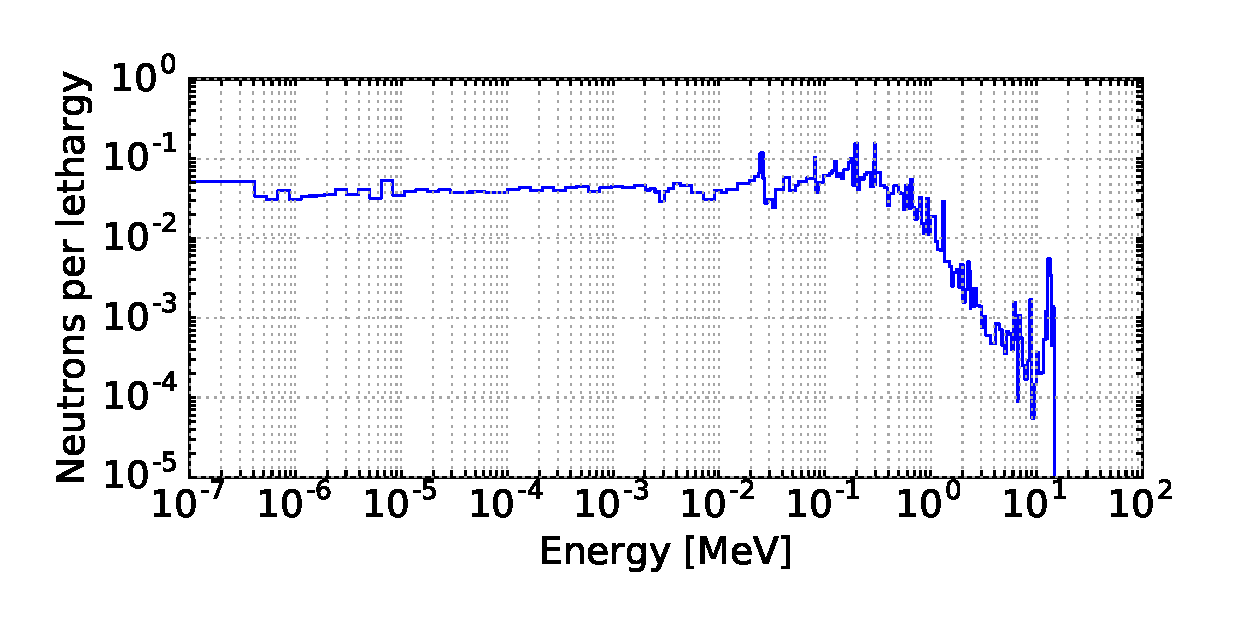
\includegraphics[width=\textwidth]{src_spectra}
  \caption{Neutron spectra for incident radiation. This spectra was tallied at back of the ITER Neutral Beam assembly.}
  \label{fig:src_spectra}
\end{figure}

\paragraph{Photon}
The Tokamak Cooling Water System (TCWS) will move large quantities of water through an intense neutron flux during ITER's operation. This water leaves the tokamak through a network of penetrations and pipes in the surrounding facility. The water is activated mainly by the following reactions: \textsuperscript{16}O(n,p)\textsuperscript{16}N and \textsuperscript{17}O(n,p)\textsuperscript{17}N. These nitrogen isotopes rapidly decay as shown in table~\ref{tab:nitrogen_decay}.

\begin{table}[H]
  \centering
  \begin{tabu} to \textwidth {X[3] X X X[5]}
    \toprule
    Activation product  & t$_{\frac{1}{2}}$(s)  & Decay mode  & Energy (MeV) [branching ratio \%] \\
    \midrule
    \textsuperscript{16}N & 7.13 & $\gamma$              & 6.129 [67], 7.115 [5] \\
    \textsuperscript{17}N & 4.14 & $\beta \rightarrow n$ & 0.383 [35], 1.171 [53] \\
    \bottomrule
  \end{tabu}
  \caption{The type, energy and likelihood of decay from activated N isotopes in the ITER water cooling system.}
  \label{tab:nitrogen_decay}
\end{table}

The gamma decay of \textsuperscript{16}N is utilised as a source for several of the simulations presented in section~\ref{subsec:prompt}.

\subsubsection{Computation}
\label{subsubsec:rad_tran_comp}
The nuclear data employed was the continuous energy Joint Evaluated Fission and Fusion file 3.2 (JEFF3.2) for neutron transport and MCPLIB84 for photon transport. EAF2010 data was used at ITER Organisation's request for activation calculations. Radiation transport was conducted with MCNP6v1.0

The MCNP relative error, $R = \frac{\sigma_{s}}{\mu_{s}}$ which is the ratio of sample standard deviation to sample mean was kept to below 0.1 for all energy bins and mesh voxels where possible. However, the wall is a shield and heavily attenuating of source particles. For a 50cm thickness of concrete, the neutron attenuation is approximately 7 orders of magnitude. Therefore in order to converge the spectrum and solve the problem a significant number of histories must be run. 

Converging results on a coarse energy grid or `group structure' requires fewer source particles for a given $R$, but having fewer energy bins means the spectrum will be correspondingly poorly resolved, with large steps in flux across the energy domain. Initial simulations using VITAMIN-J 175 group structure did a good job of resolving the spectrum from 1 eV up to the fusion peak at 14MeV, however they completely fail to represent the fine structure of the thermal spectrum. This is demonstrated in figure~\ref{fig:neutron_group_comparison}. The two lowest bins are $[10^{-5},10^{-1})$ eV and $[10^{-1},4.1\times10^{-1})$ eV. Despite the lack of thermal energy resolution, VITAMIN-J extends to very low energies. This means that neutrons scored at thermal energies contribute equally across four orders of magnitude in the lowest bin. When a spectrum such as this is sampled later, for an activation calculation, say, fictitious neutrons at $10^{-5}$ and $10^{-4}$ eV are produced and will skew results for problems where reactions in the 1/E region are significant, potentially drastically overestimating reaction rates. 

\begin{figure}[H]
  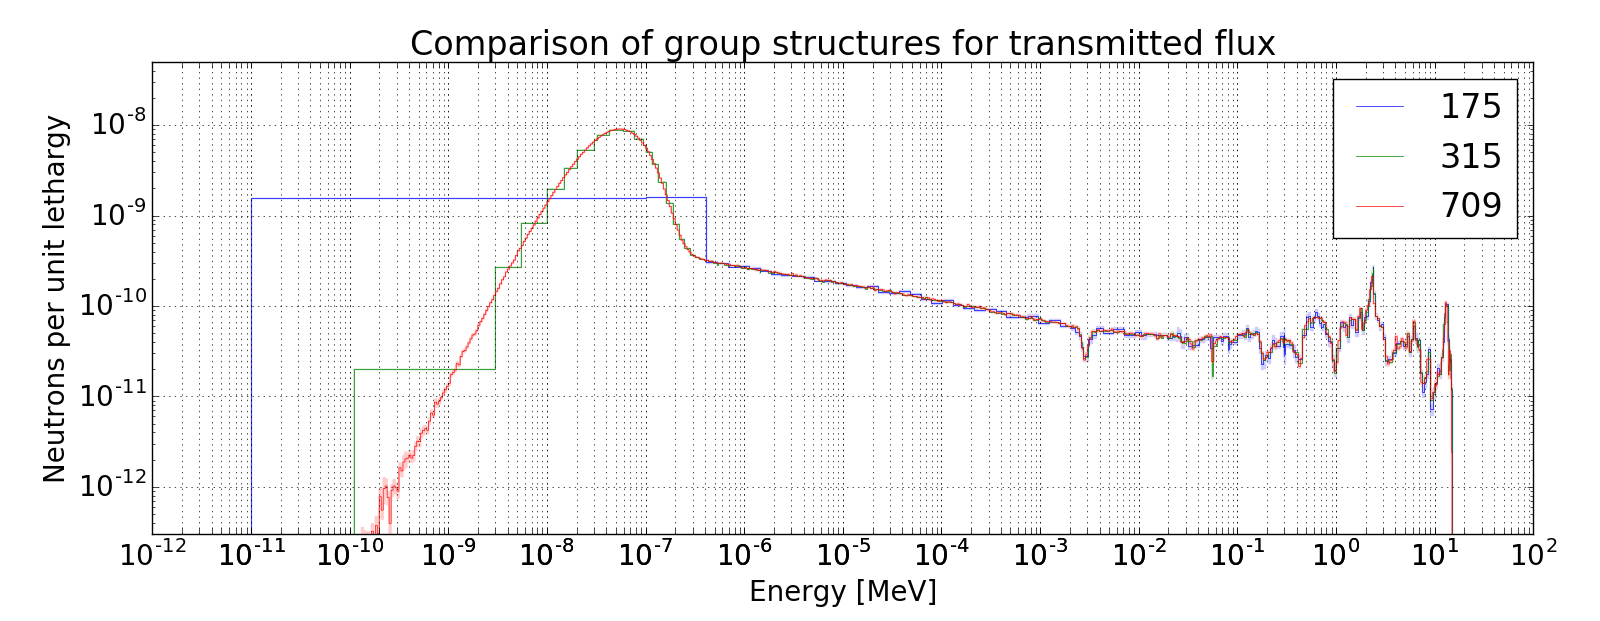
\includegraphics[width=\textwidth]{shield_flux_by_group.png}
  \caption{This figure shows the same transmitted flux, as simulated by MCNP, binned in a variety of group structures. While the region down to approximately 1 eV is resolved broadly similarly, the VITAMIN-J 175 group structure has insufficient bins to resolve a Maxwellian distribution of thermal neutrons in the low-energy region.}
  \label{fig:neutron_group_comparison}
\end{figure}

The ideal group structure should contain enough bins in the low energy region to approximate a thermal distribution. However, as previously stated, all bins should converge to have a relative error of less than 0.1 as proof of convergence. For this particular problem, convergence is most difficult for the high energy region, as these particles are relatively rare. Hence, many fine bins in the high energy region will necessitate significantly longer run times. For the work presented here, the 315 neutron group structure was selected as a compromise between speed and fidelity.

%\begin{equation}
%\lambda_{D(e)}=\sqrt{ \frac{ \varepsilon_0 k_B T_{(e)}}{e^2 n_\infty}}
%\end{equation}

\subsection{Shut Down Dose Rate (SDDR)}
The calculation of $\phi_{\gamma}(x,y,z,E,t)$ where $t$ is some time after cessation of plasma operation comprises three main steps:
\begin{enumerate}
  \item 1) Neutron transport---as previously, compute the neutron flux during plasma operation, $\phi_{n}(x,y,z,E)$, recording the neutron flux binned by energy over a spatial mesh. Finer meshes will converge on true behaviour, with coarse meshes over or under-estimating fluxes depending on local geometry and flux gradients \footnote{Using a mesh which conforms to the geometry, such as an unstructured mesh has been shown to give significant improvements, especially for small features \cite{Eade2015}.}.
  \item 2) Activation---determine the appropriate irradiation scenario, then activate and transmutate the materials present in the problem geometry. This involves assembling a system of differential equations, Bateman equations, to track the inventory of all the nuclides present. One can numerically solving this system for a series of timesteps using codes such as FISPACT-II \cite{sublet2017a}. The resulting nuclides and their abundances can be paired with decay data to generate a decay photon source on the original mesh. 
  \item 3) Photon transport---using the distributed decay gamma source produced by step 2), conduct a radiation transport run to determine the photon flux, $\phi_{\gamma}(x,y,z,E,t)$, converting to effective dose as required.
\end{enumerate}

\subsubsection{Model geometry}
The shut-down dose rate is calculated for the following scenario: it assumes a worker is inside the bioshield at ITER during a shutdown, stood 30cm from the inner surface of a 150cm thick wall with a steel mass fraction of 4.5\% the total wall mass. Reinforcing bar forms a mesh of squares 20cm in width and height at the front and back of the wall, 5cm from the surfaces. 

\subsubsection{Materials}
For analysis of the SDDR, where small impurities can have large contributions to the dose rate, the steel composition was refined \cite{Barabash16}. ITER limits for Co and Ni were imposed, 0.01\%wt and 0.05\%wt respectively. The resulting composition for steel is shown as table~\ref{tab:sddr_steel}.

\begin{table}[H]
  \centering
  \begin{tabu} to 0.3\textwidth {X X}
    \toprule
    Element & \% weight \\
    \midrule
    Fe & 97.613 \\
    C  & 0.22 \\
    P  & 0.05 \\
    S  & 0.05 \\
    N  & 0.012 \\
    Mn & 1.08 \\
    Cr & 0.1 \\
    Mo & 0.01 \\ 
    V  & 0.005 \\
    Ni & 0.05 \\
    Cu & 0.8 \\
    Co & 0.01 \\
    \bottomrule
  \end{tabu}
  \caption{Steel composition \% weight for SDDR calculations from \cite{Barabash16}. This composition includes minor constituents which are not important for radiation transport, but may play a significant role in any SDDR.}
  \label{tab:sddr_steel}
\end{table}

\subsubsection{Computation}
As for before, radiation transport was conducted with MCNP6 v1.0. Neutron spectra were tallied on a mesh in the shield models. These spectra were used as input to the MCR2S activation linker code \cite{Davis2010a}. This program uses these spectra and a corresponding irradiation scenario to compute material changes within the meshed model. These new materials and decay information can be used to generate a photon source from the activated nuclides. The final steps in the calculation are to perform photon transport calculations from the activated wall to a target. The generation of photon sources and transport of emitted $\gamma$-rays must be computed for each decay time step of interest.

The irradiation scenario employed for the activation step was ITER's SA-2 \cite{Loughlin09}, which approximates the ITER DT experimental programme total fluence and explicitly includes the final, end-of-life pulses for accurate estimation of short-lived nuclides.

As noted in section~\ref{subsubsec:rad_tran_comp}, the choice of energy group structure can be important for the accuracy of calculations. When a pre-sampled neutron flux is later sampled to calculate a SDDR dose, the 175 group structure introduced a 20\% increase in dose rate for steel at all time steps, and approximately the same increase for concrete until days after irradiation, when the discrepancy between 175 and 315 falls to zero.

The dominant contributors to dose rate in steel all originate through (n,$\gamma$) and as such are not threshold reactions, instead observing 1/E behaviour at low energies. Whilst the dominant contributor to dose rate in concrete is initially \textsuperscript{24}Na formed though \textsuperscript{23}Na(n,$\gamma$)\textsuperscript{24}Na, it decays with t$_{\frac{1}{2}}=15$h before the dominant nuclide becomes \textsuperscript{39}Ar, which is produced via \textsuperscript{39}K(n,p)\textsuperscript{39}Ar. The (n,p) reaction is threshold, i.e. not effected by the low energy inaccuracy introduced by binning in 175. Therefore after a few days, the SDDR discrepancy between groups reduces to zero.

Further enquiry into the optimum energy group structures for activation calculations is presented as chapter~\ref{chap:group_structure}.

%%%%%%%%%%%%%%%%%%%%%%%%%%
% RESULTS AND DISCUSSION %
%%%%%%%%%%%%%%%%%%%%%%%%%%
\section{Results \& discussion}
This section details the effect of spatial homogenisation on fluence and dose received by workers in several circumstances. First, on-load radiation: neutrons originating from the plasma and multiplication reactions within the reactor and photons emitted from neutron induced reactions such as inelastic scattering and activation of nitrogen in water. Subsequently, a case is investigated where neutrons are transported through the shielding wall, activate it and then the resulting gamma-rays transported, this time tallied on the inner side of the wall--estimating the dose received by workers performing a maintenance action between plasma shots.

\subsection{Transmission of prompt radiation}
\label{subsec:prompt}
The transmitted, or `leakage' neutron spectra for a thick (2.1m) concrete wall is shown below as figure~\ref{fig:trans_neutron_spec}. Note the DT and prominent DD reaction peaks at 14.1 and 2.5 MeV respectively. Other features are the flat slowing-down region with a few flux depressions and the significant thermal Maxwellian distribution. The flux has been severely reduced by its interaction with the wall, decreasing from the source by an order of magnitude each 20cm traversed. The most prominent difference between the heterogeneous and homogeneous models is in the thermal region. 

\begin{figure}[h]
  \centering
  \figuretitle{Transmitted neutron spectra}
  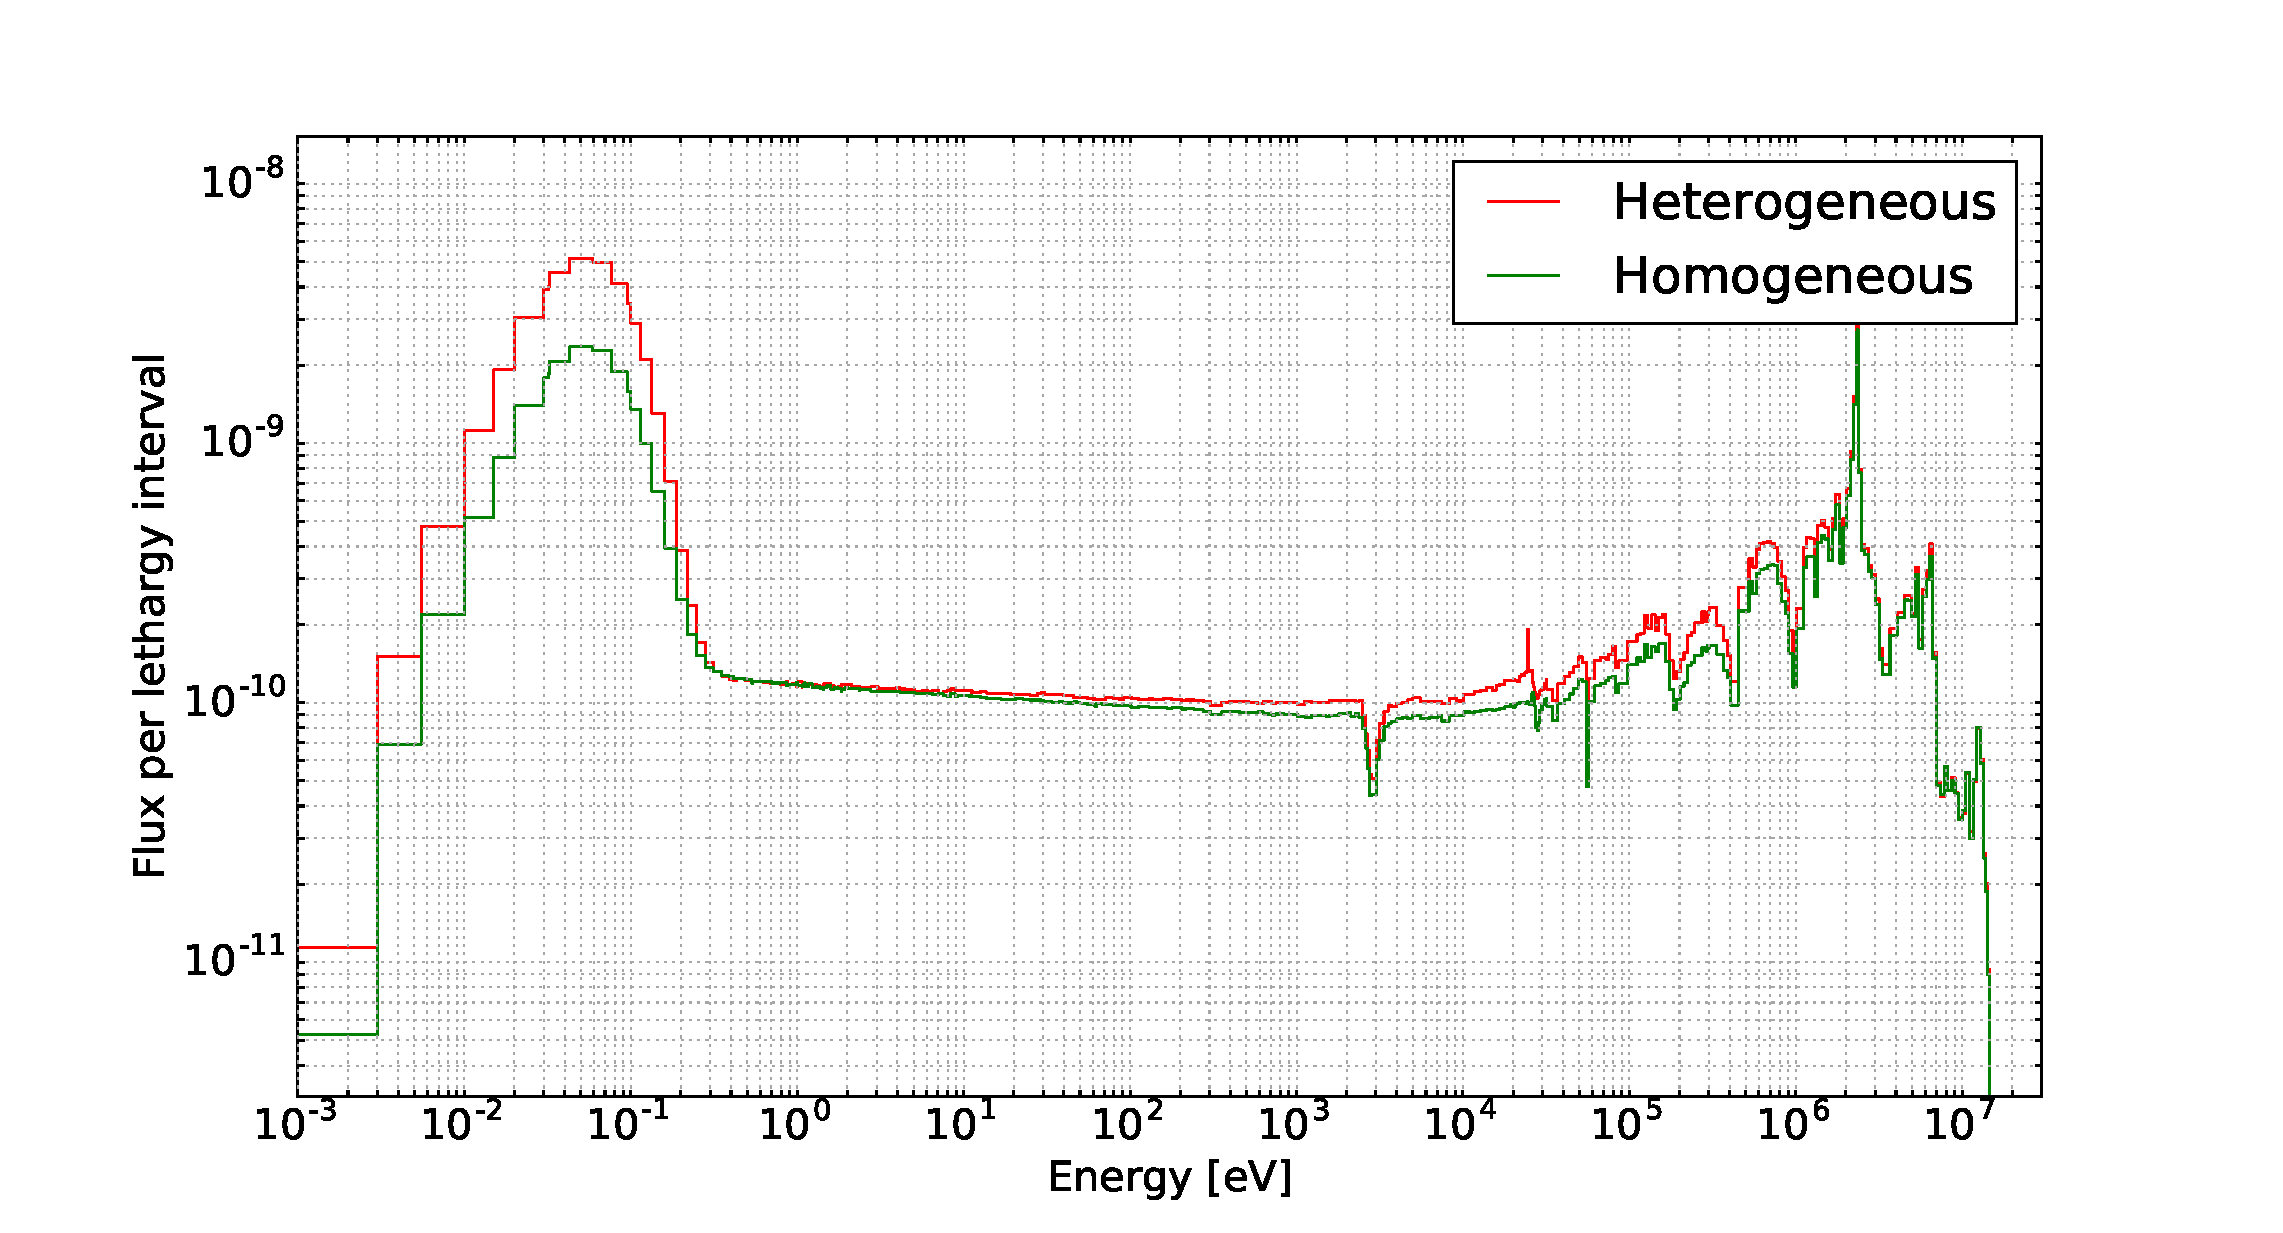
\includegraphics[width=0.9\textwidth]{transmitted_neutron_spectra}
  \caption{The neutron spectra leaving the shield for the heterogeneous and homogeneously modelled cases. This example is for the thickest wall simulated, at 2.1m thickness. The rebar is 41mm in diameter at 200mm spacing, resulting in a steel mass fraction of 4.45\% of the shield total. Note the substantially reduced thermal flux in the homogeneous simulation. The spectrum has been binned with the TRIPOLI 315 group structure.}
  \label{fig:trans_neutron_spec}
\end{figure}

The reduced transmitted homogeneous thermal flux in figure~\ref{fig:trans_neutron_spec} is in part because steel is now available for neutron interactions throughout the depth of the wall, in the homogenised material, rather than solely being available for interactions near the surfaces. Steel has a greater macroscopic material capture cross-section than concrete, and so acts as a neutron sink for slow neutrons, preventing them from propagating through the shield. The material cross-sections for radiative capture are shown in figure~\ref{fig:n_rad_capture}.

\begin{figure}[h]
  \centering
  \figuretitle{Radiative capture probability}
  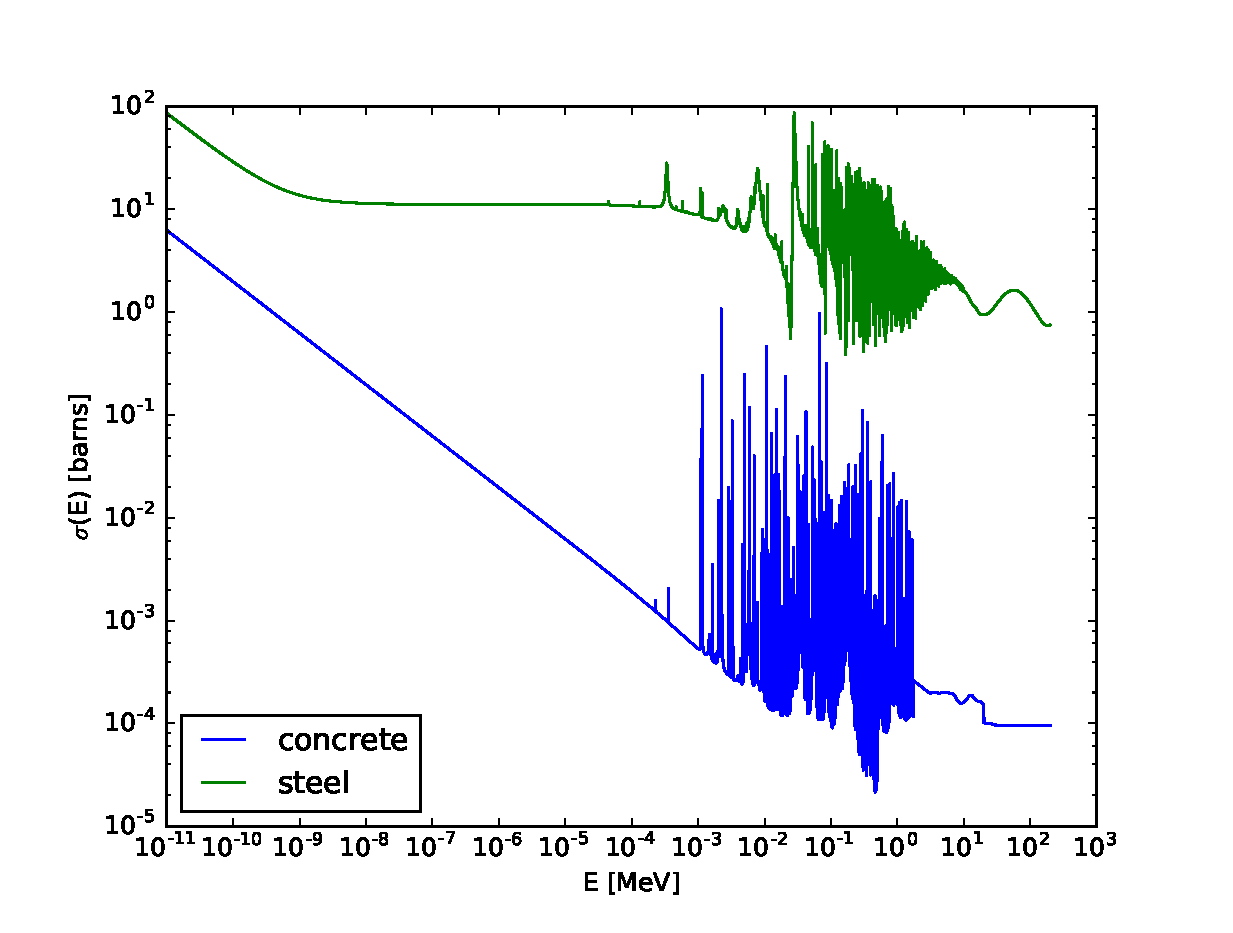
\includegraphics[width=0.8\textwidth]{n_rad_capture}
  \caption{The nuclear properties of steel and concrete are substantially different. Shown here is the cross-section for $(n,\gamma)$ in both materials. At thermal energies steel has a material radiative capture cross-section two orders of magnitude greater than concrete.}
  \label{fig:n_rad_capture}
\end{figure}

Plotting the ratio of the leakage neutron spectra as figure~\ref{fig:relative_neutron_spectra}, one can see the differences in flux more easily. Thermal flux is underestimated by more than a factor 2. But also, fast flux in the 1keV--1MeV range is underestimated by $\sim1.2$. The fast flux discrepancy is correlated with wall thickness and is negligible for thin (\textless 1m) walls.

\begin{figure}[h]
  \centering
  \figuretitle{Relative neutron spectra}
  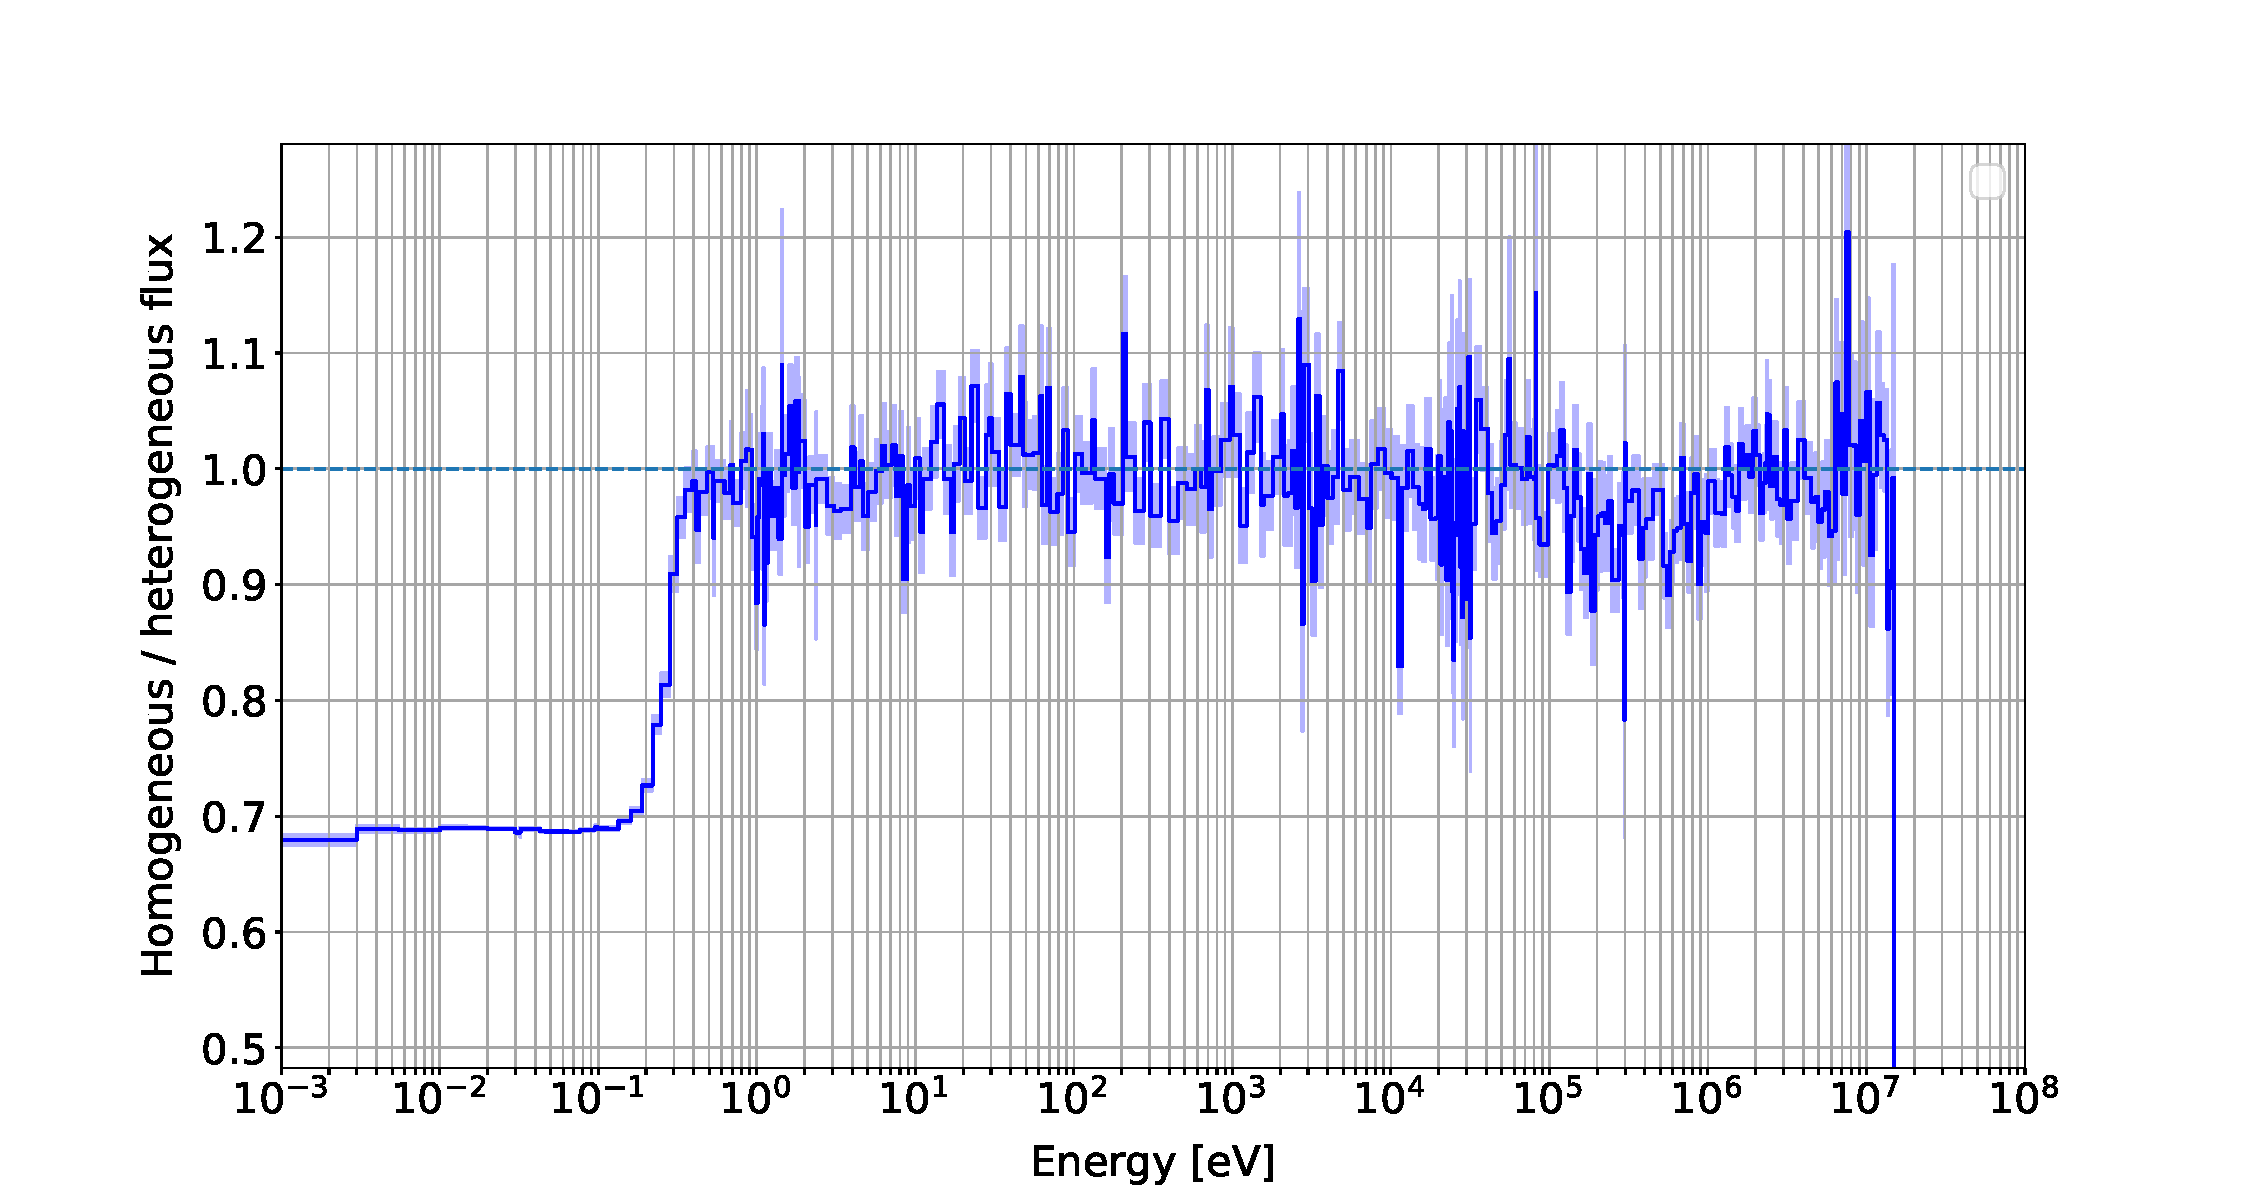
\includegraphics[width=0.8\textwidth]{25HB200_800_relative_n_spectra}
  \caption{The homogeneous flux increases are readily visible in this example. The ratio is of the two spectra from figure~\ref{fig:trans_neutron_spec}. Errors have been combined in quadrature and are plotted as the light shading surrounding the mean value.}
  \label{fig:relative_neutron_spectra}
\end{figure}

Figure~\ref{fig:dose_discrepancy} shows how the received dose discrepancy due to the homogeneous approximation varies with wall thickness. Thin walls have a relatively small discrepancy--to be expected as the heterogeneous model is at its most similar to the homogeneous in this case. As the walls become thicker and the rebar meshes become separated by a larger volume of concrete, the discrepancy increases. It plateaus at $\sim 1m$ wall thickness. Similar behaviour is observed for dose due to prompt photons. It can be seen that the effect is greatest for neutrons, with a maximum dose underestimate of 22\%.

\begin{figure}[h]
  \centering
  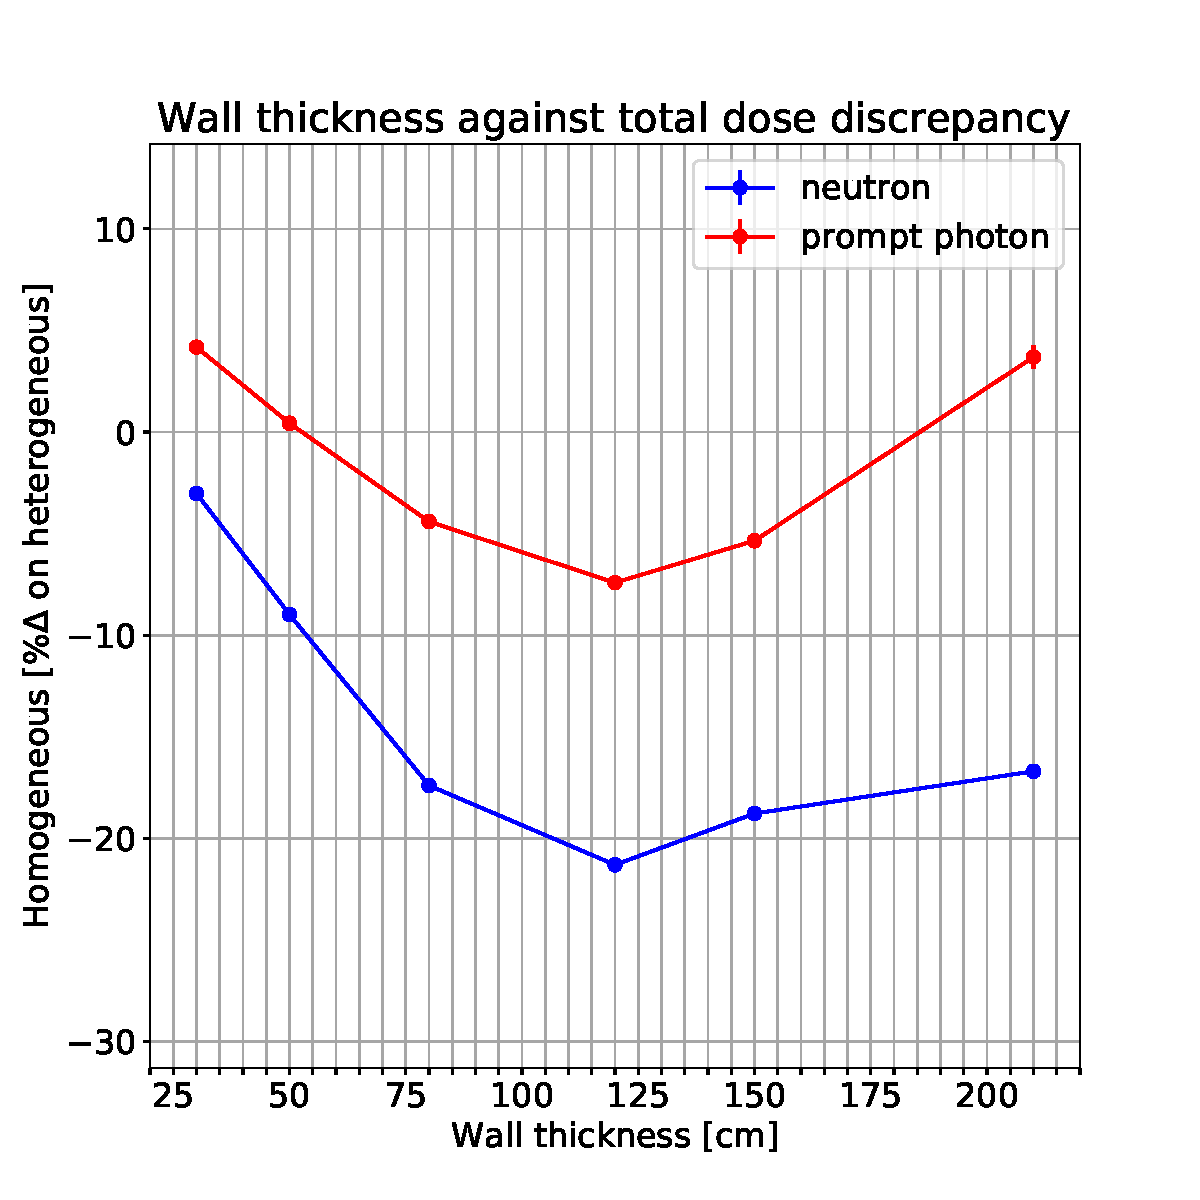
\includegraphics[width=0.7\textwidth]{wall_thickness}
  \caption{This figure shows the relationship between the wall thickness and the difference between the homogeneous and heterogeneously modelled walls. The quantity plotted is the energy integrated dose for each case, for neutrons and prompt photons. Error bars due to radiation transport statistics are shown but may not be visible on this scale. The discrepancy between modelling approaches is a function of the wall thickness, greater for neutrons than photons.}
  \label{fig:dose_discrepancy}
\end{figure}

\FloatBarrier
\subsection{Shut Down Dose Rate (SDDR)}
\label{subsec:sddr}
After operation of a tokamak, repairs and maintenance are often necessary. This section explores the shut-down dose due to be received from the wall itself. It assumes a worker is inside the bioshield at ITER during a shutdown, stood 30cm from the inner surface of a 150cm thick wall with a steel mass fraction of 4.5\% the total wall mass. Reinforcing bar forms a mesh of squares 20cm in width and height at the front and back of the wall, 5cm from the surfaces. Dose rates due to neutron activation in the reinforced concrete shielding have been calculated for when the reinforced conrete is homogenised and when it is modelled faithfully.

The effect of the spatial homogenisation modelling approximation generally acts to overestimate the SDDR by a small amount. The behaviour is shown as figure~\ref{fig:sddr}. On the timescale of seconds and minutes, and from days out to decades, the overestimate is approximately 10\%. On the timescale of hours, the discrepancy between homogeneous and heterogeneous approaches closes, briefly becoming reversed, with the homogeneous approximation underestimating the SDDR by 4\%. The absolute dose due to photons from the reinforced wall will have fallen by an order of magnitude in the period elapsed between a minute and a week after the final DT shot and it is unlikely anyone will be entering the facility before then.

\begin{figure}[h]
  \centering
  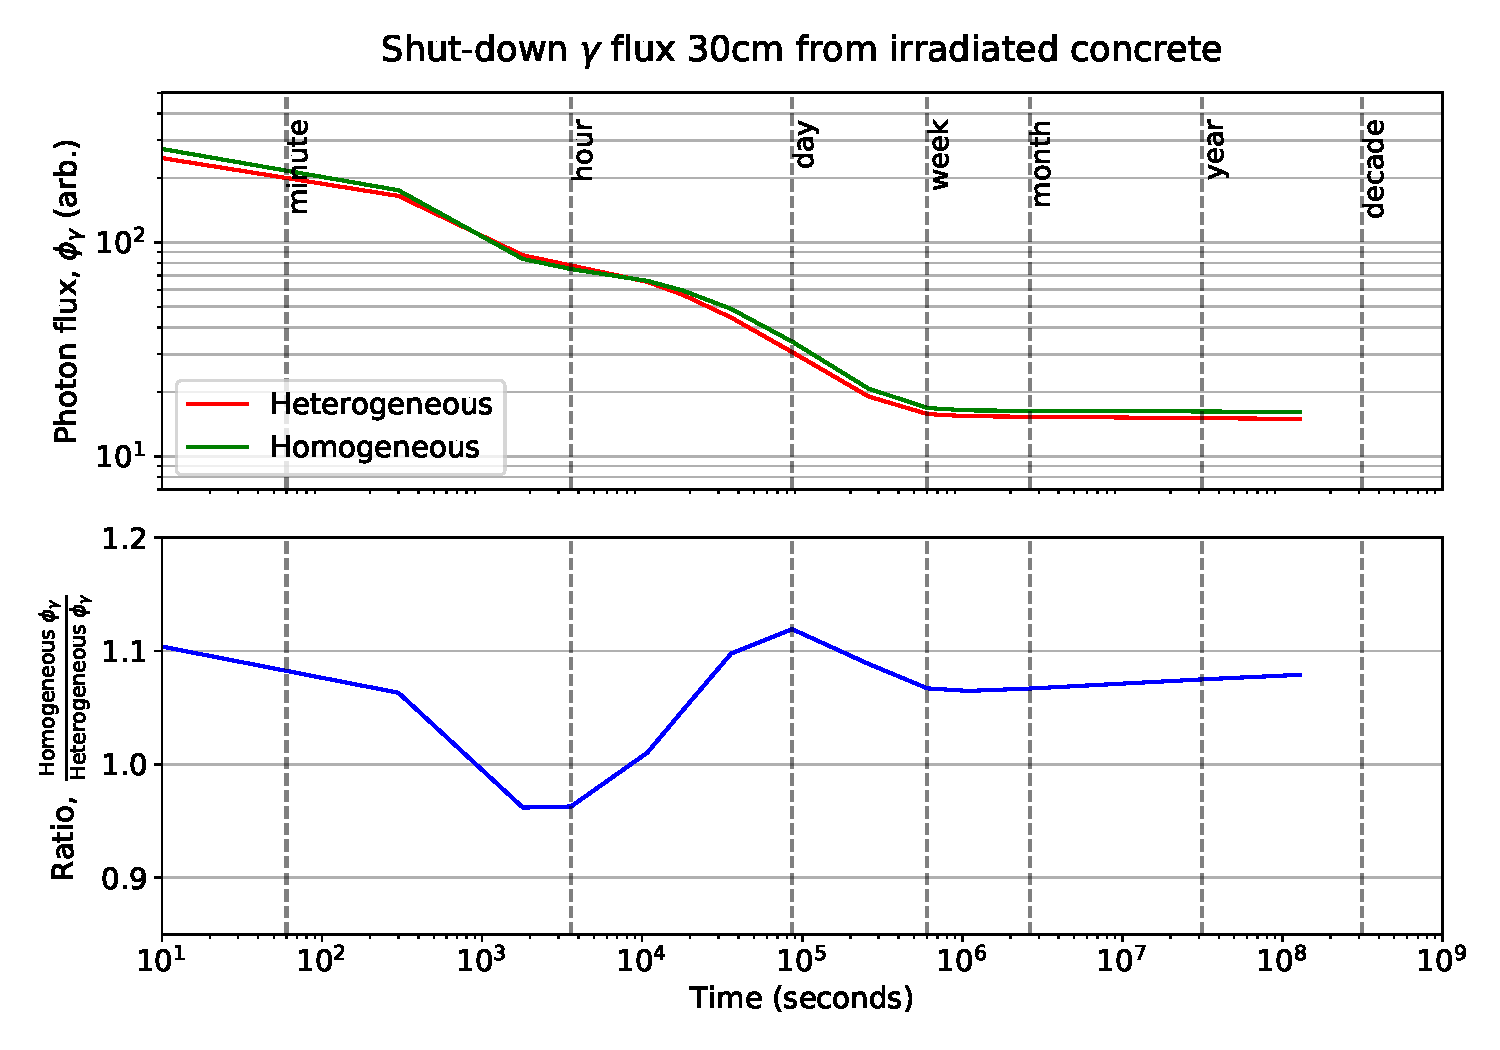
\includegraphics[width=0.8\textwidth]{sddr}
  \caption{This figure displays total $\phi_{\gamma}$ received at a distance of 30cm from the activated wall. The upper panel displays the absolute values in the heterogeneous and homogeneous modelling approaches, as a function of time since last irradiation. There are 16 time steps, for which the activation and subsequent photon transport has been carried out. The lower panel displays the ratio between the approaches, i.e. homogeneous values normalised by the heterogeneous values. One can see that the homogeneous approximation artificially increases the SDDR by $\approx 10\%$ at most time steps, bar those around an hour.}
  \label{fig:sddr}
\end{figure}

The complex behaviour displayed in figure~\ref{fig:sddr} is a result of the many different nuclides which contribute to the decay $\gamma$ field. These nuclides have a range of half-lives and inspecting their relative emissions as a function of time is instructive in understanding the shape of figure~\ref{fig:sddr}. The plot shown as figure~\ref{fig:contact_dose} displays estimates for a contact dose with concrete and steel. As the steel is buried within concrete, the numbers plotted here are not a substitute for transporting decay $\gamma$ photons from their emission to their absorption. However, figure~\ref{fig:contact_dose} does give a good feel for which nuclides are responsible for the activity of each material at a given time. 

\begin{figure}[h]
  \centering
  \figuretitle{Contact dose rate by material}
  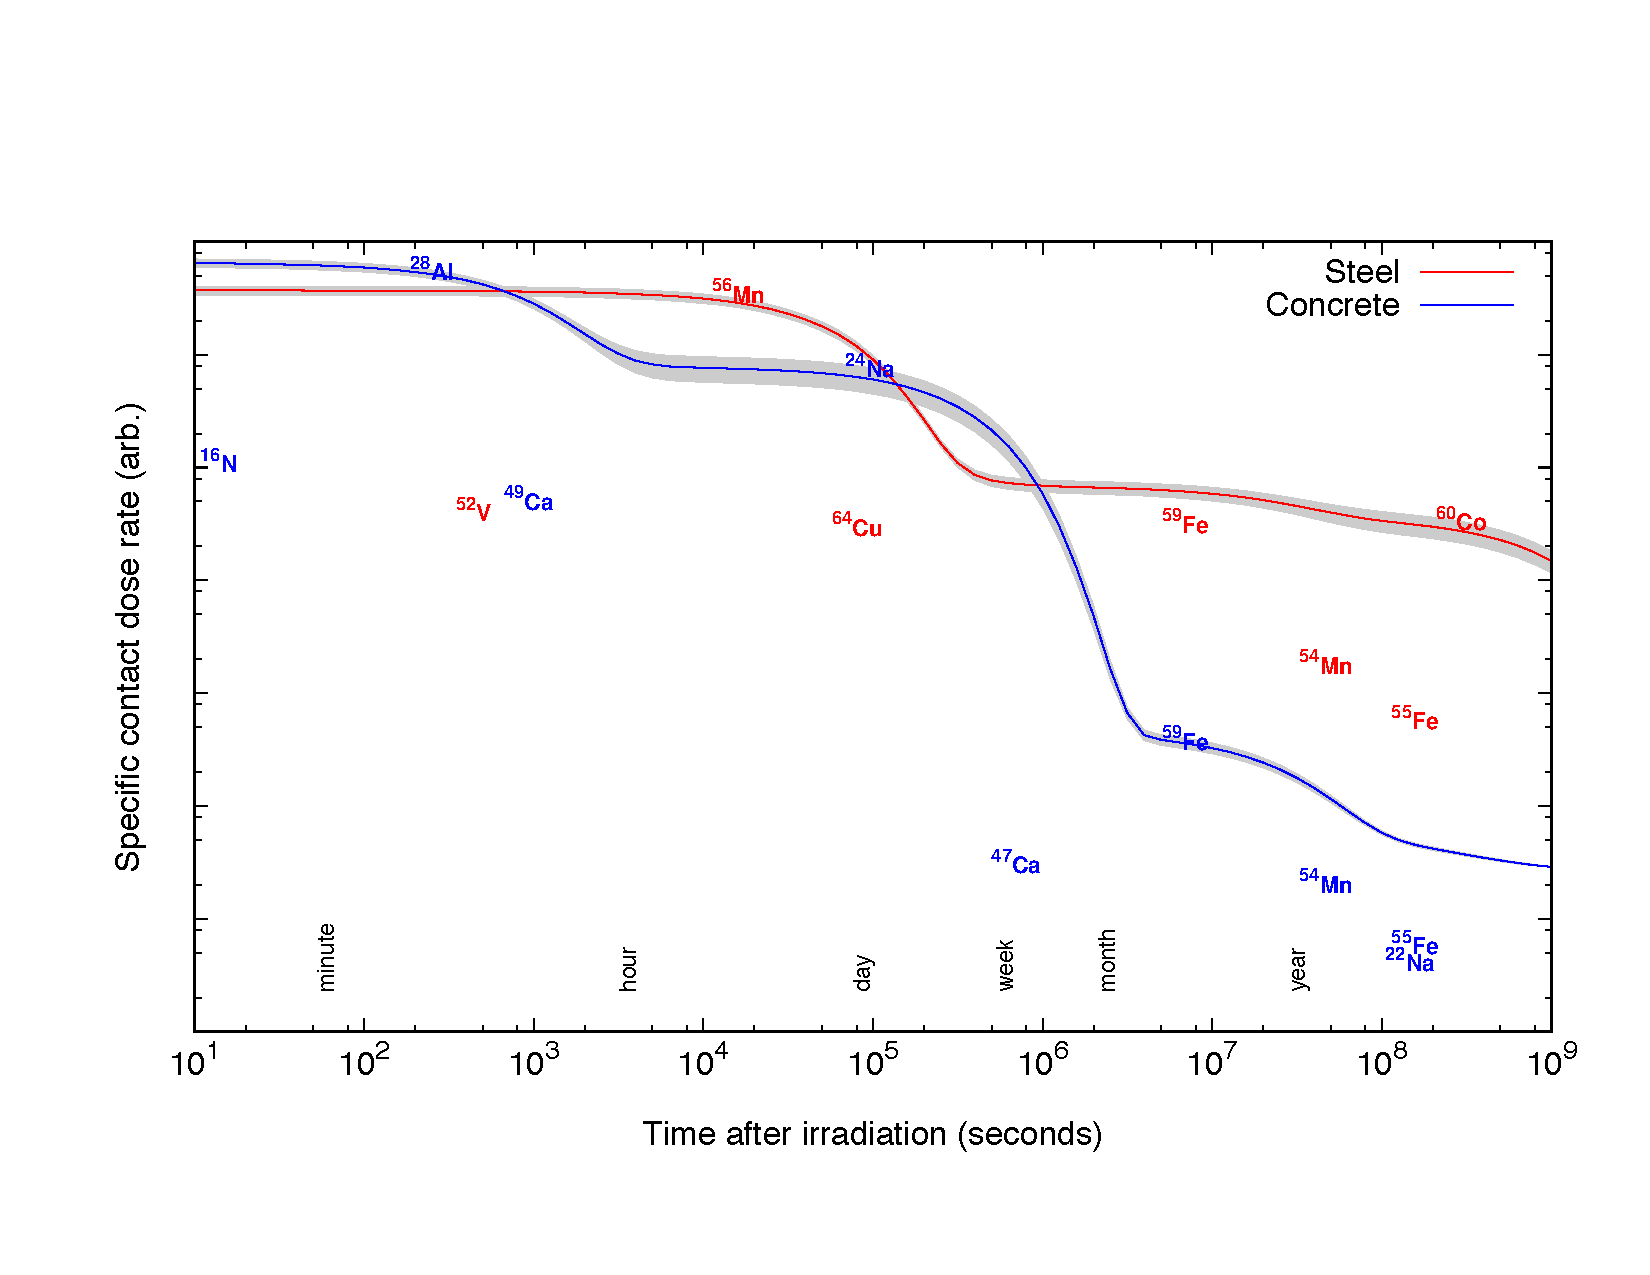
\includegraphics[width=0.8\textwidth]{contact_dose_by_mat}
  \caption{This plot shows an estimate for the specific contact dose rate due to steel and concrete irradiated under the ITER SA-2 scenario. The total specific dose rate is given by the line plots, with an uncertainty band from EAF-2010 data included as the grey shading. Nuclides which contribute a significant fraction of the dose are shown with their abscissa value as their half-life, $t_{\frac{1}{2}}$ and their ordinate as their contribution to the specific dose rate. The specific dose rate behaviour is quite complex; the material with the highest specific activity changes three times in the simulation period due to various decays.}
  \label{fig:contact_dose}
\end{figure}

From figure~\ref{fig:contact_dose} it is clear that the two materials clearly have quite different nuclear properties, so it is not surprising that their spatial distribution influences the dose received. On a per-mass basis, concrete is more active on the timescale of minutes due to $^{28}$Al. Subsequently, until a few hours have elapsed since last irradiation, gamma emission from $^{56}$Mn makes steel the most active. $^{24}$Na then makes concrete the most active on the timescale of days and after its decay, steel becomes dominant out to very long timescales. The period around an hour or two, where $^{56}$Mn is the dominant nuclide in steel, is also where the homogeneous modelling approach briefly stops overestimating the dose due to the shut-down $\gamma$ field. %This could be connected, $^{56}$Mn undergoes $\beta^{-}$ decay followed by gamma emission of 0.85, 1.81 \& 2.11 MeV energies to become stable $^{56}$Fe. 

\begin{figure}[h]
  \centering
  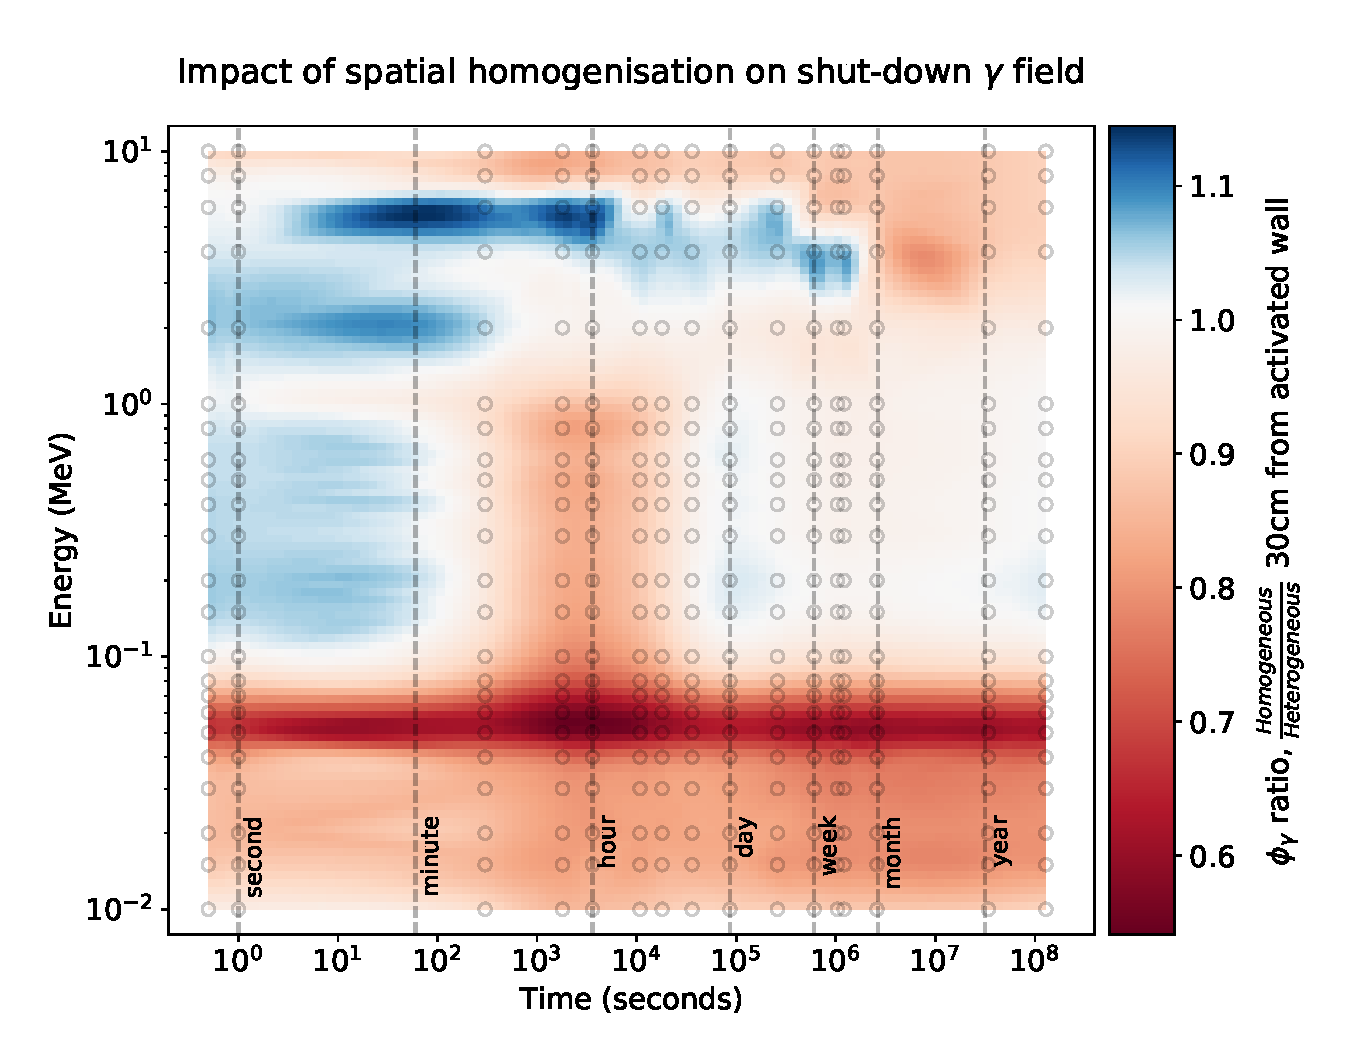
\includegraphics[width=0.8\textwidth]{sddr_nrg.pdf}
  \caption{This figure displays the ratio of homogeneous and heterogeneous $\phi_{\gamma}$ fluxes for a series of cooling times and all photon emission energies. Time since last irradiation is given in seconds on the abscissa, while the ordinate is photon emission energy in MeV. The grey circles indicate simulation data, i.e. flux ratios for a particular photon energy group at a particular cooling timestep. These data have been interpolated with a cubic method to generate the heatmap shown. A diverging colourmap helps identify where spatial homogenisation is overestimating dose (blue) and where it underestimates (red).}
  \label{fig:sddr_nrg}
\end{figure}

Homogeneous simulations tend to overestimate the number of high-energy gamma photons, as some steel material is located everywhere in the homogenised mixture, including the shallow volume, outside of where the rebar is located in the heterogeneous models. This steel lying on the surface in the homogeneous model will emit high-energy, gamma rays which can leave the shielding unattenuated and are more likely to contribute to a worker's dose\footnote{High energy, $1 < \mathrm{E [MeV]} < 2$ gamma-rays constitute the majority of the dose received at all times, however beyond 2 MeV the flux and contribution to dose falls off sharply.}. This behavior is shown in figure~\ref{fig:sddr_nrg} where the ratio of homogeneous and heterogeneous gamma spectra have been plotted for a variety of timesteps. Work to corroborate this explanation could include varying the cover depth, to see if homogeneous models started to underestimate the received dose as the cover depth approached zero and the rebar was on the surface in the heterogeneous model.

% The mean free path of neutrons near the surface is $\sim2cm$ (see figure \ref{fig:mfp}) and as such a typical neutron will undergo several collisions before arriving at the rebar in a heterogeneous simulation. However, in a homogeneous simulation a small amount of steel is present right at the very surface of the concrete, as it is present throughout the simulation. This steel is exposed to an intense neutron flux and is activated accordingly.

% \begin{figure}[h]
%   \centering
%   \figuretitle{Neutron path length in concrete}
%   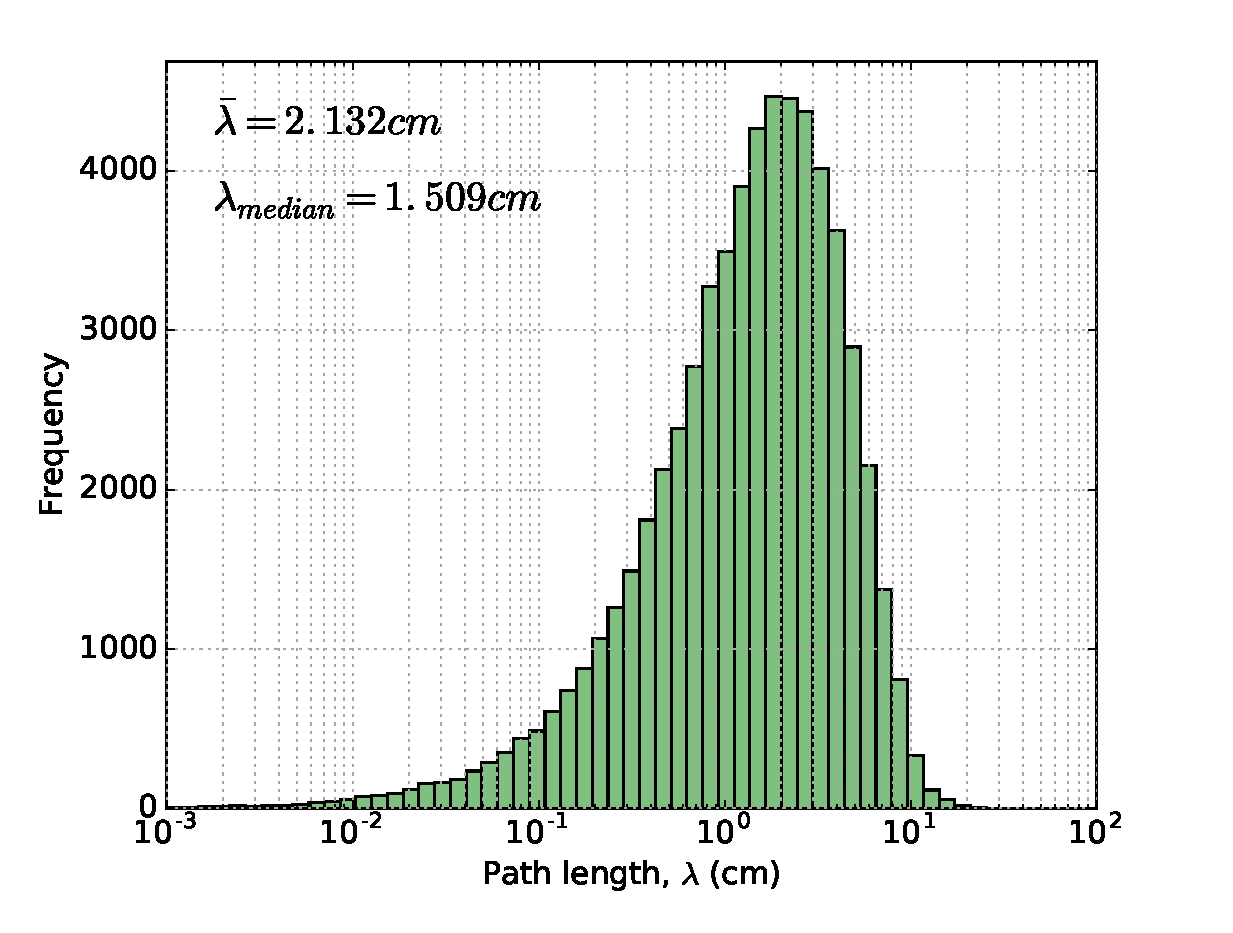
\includegraphics[width=\textwidth]{mfp}
%   \caption{The path lengths of neutrons in pure concrete are shown as a histogram. There is a wide distribution with a mean of approximately 2cm.}
%   \label{fig:mfp}
% \end{figure}

\FloatBarrier
\section{Conclusion}
The spatial homogenisation modelling approximation for reinforced concrete underestimates the dose due to neutrons by up to 20\%. The dose due to on-load photons can be underestimated by up to 8\%. The SDDR is instead overestimated by homogenisation, by up to a factor 60 at times beyond a day. 
